\documentclass[a4paper,twoside,11pt]{article}
\usepackage[utf8]{inputenc}
\usepackage[english]{babel}
\usepackage{graphicx}
\usepackage{url}
\usepackage{float}

% pdflatex

% redefinição das margens das páginas
\setlength{\textheight}{24.00cm}
\setlength{\textwidth}{15.50cm}
\setlength{\topmargin}{0.35cm}
\setlength{\headheight}{0cm}
\setlength{\headsep}{0cm}
\setlength{\oddsidemargin}{0.25cm}
\setlength{\evensidemargin}{0.25cm}
\setlength{\textfloatsep}{16pt}

\begin{document}

\begin{figure}[t]
\centering

\includegraphics [width=5in]{logoISEL.png}
\end{figure}

\title{\huge \textbf{WaveCoach}\\[1ex]\LARGE Training Management Platform for Surf}

\author{
\begin{tabular}{c}
             Tiago Canilhas, n.º50472, e-mail: a50472@alunos.isel.pt, tel.: 924115540\\
             João Barrisco, n.º50476, e-mail: a50476@alunos.isel.pt, tel.: 967487235\\
\end{tabular}}

\date{
\begin{tabular}{ll}
  {Supervisor:} Filipe Freitas, e-mail: ffreitas@cc.isel.ipl.pt \\
\end{tabular}\\
\vspace{5mm}
April 28,  2025}

\maketitle

\section{Introduction}
The goal of this project is to develop a web application that allows the management of surfing athletes. This application is mainly aimed at coaches, but athletes can also access it to view their performance. Coaches will be able to register athletes, log different training sessions (e.g. gym, surf), record competition results, and monitor
performance through interactive charts. This will help them analyze progress and adjust training plans. This project is being developed to meet coaches' need for a more efficient and effective platform, replacing manual registration, which can be time-consuming and difficult to manage as the number of athletes grows. The platform not only saves time but also ensures greater accuracy and accessibility of data, allowing coaches to focus more on their athletes’ development and less on administrative tasks.

The project has already been initiated, and certain functionalities have already been developed, such as user registration, athlete management, and the athlete profile.

\section{Accomplished Tasks}


\subsection{Backend}

\subsubsection{Technologies}
\begin{itemize}
\item Kotlin
\item Spring Framework
\item Java Database Interface (JDBI)
\item PostgresSQL
\end{itemize}

\subsubsection{Entitity Relationship Model}

\begin{figure}[H]
\centering
\includegraphics[width=6in]{EA.png}
\caption{Entity Relationship Model}
\end{figure}

\subsubsection{Backend Organization}
\begin{figure}[H]
\centering
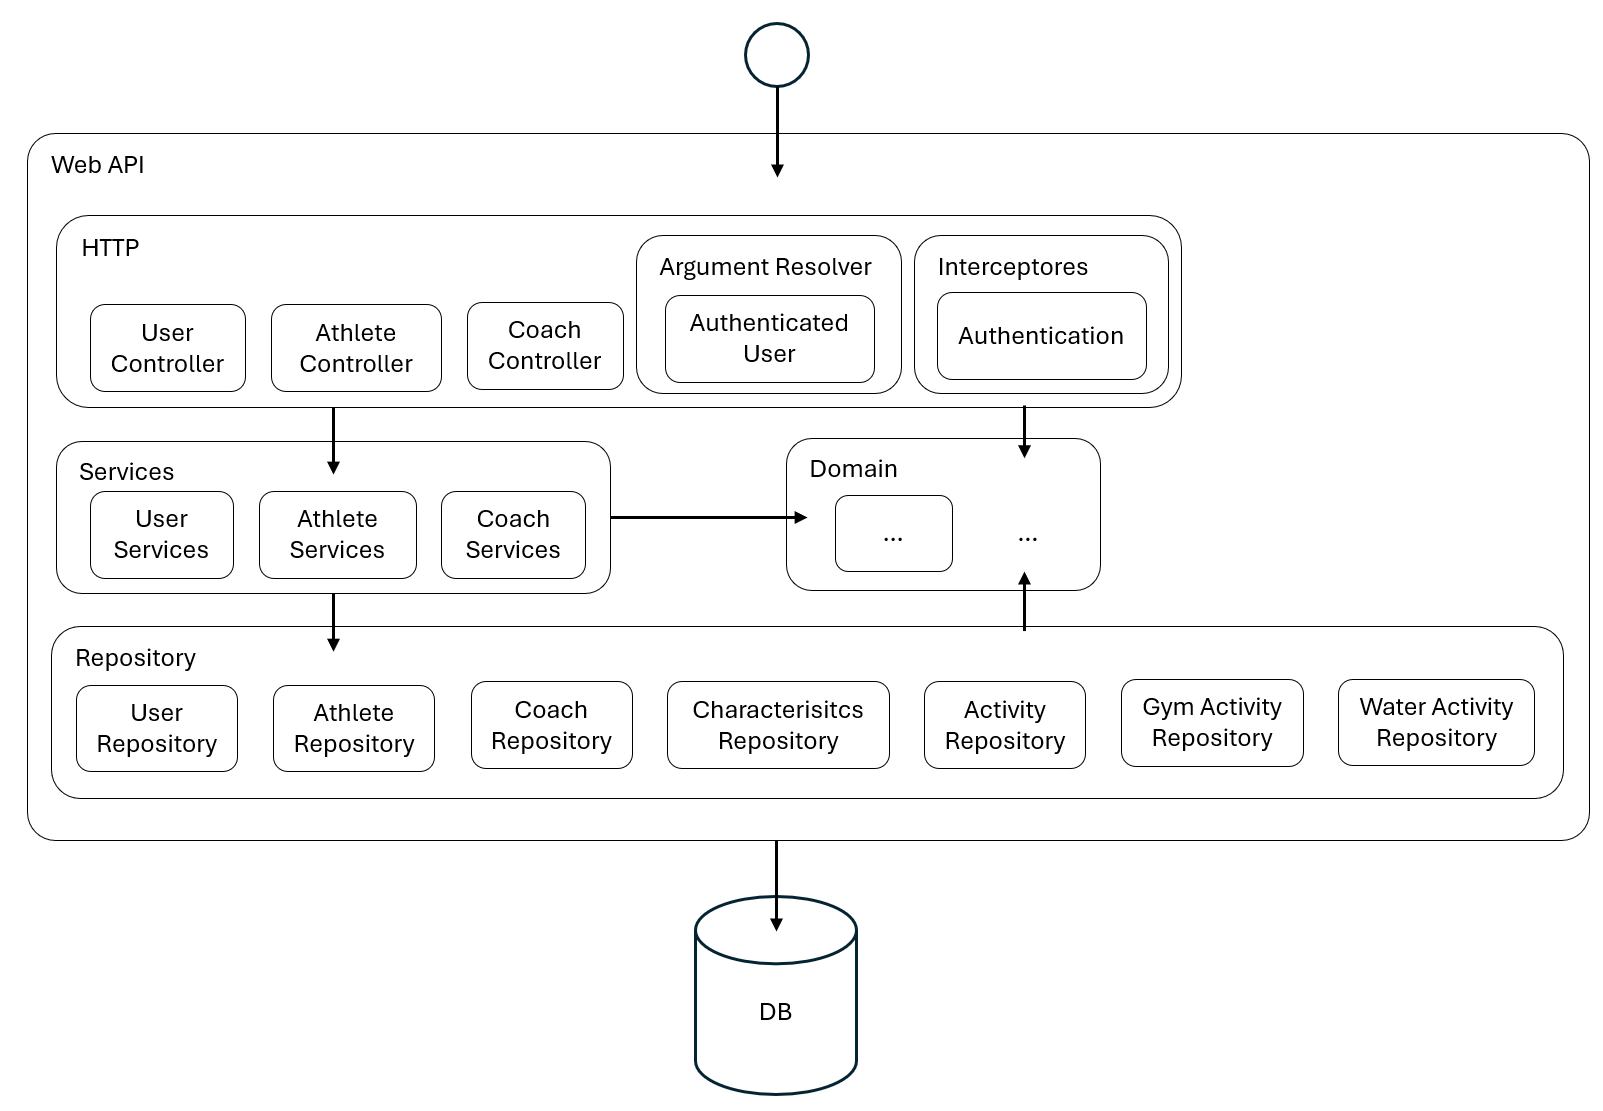
\includegraphics[width=6in]{BackendDiagram.png}
\caption{Backend Diagram}
\end{figure}

\subsubsection{Functionalities:}
\begin{itemize}
\item User Registration and Login - 
One of the first functionalities to be implemented was user registration. This is divided into two parts: athlete registration and coach registration. The athlete registration consists of two steps: first, the athlete enters a code that was provided by the coach, and second, the athlete adds their credentials, that is, a username and password. This process exists because our application is mainly aimed at coaches, meaning that, in order for coaches to easily and quickly add their athletes, the athletes do not need to have registered beforehand. Coach registration is simpler, requiring only a username and password. After the registration process was completed, the login functionality was then implemented.

No backend, para implementar estas funcionalidades... tendo sido, por fim, realizado testes para todas as funções criadas.

\item Athlete management - 
After user registration and login, aspects related to athlete management were developed, including the coach's functionalities to retrieve, add, update, and remove their athletes. All of these functionalities were thoroughly tested.

\item Athlete Profile - 
Finally, some functionalities related to the athlete were developed, such as the characteristics feature, where the functionalities to retrieve, add, update, and remove the athlete's characteristics were created and tested.

\end{itemize}

\subsection{Frontend}

\subsubsection{Technologies}
\begin{itemize}
\item Typescript
\item React
\item CSS Module
\item Webpack
\end{itemize}

\subsubsection{Frontend Organization}

\begin{figure}[H]
\centering
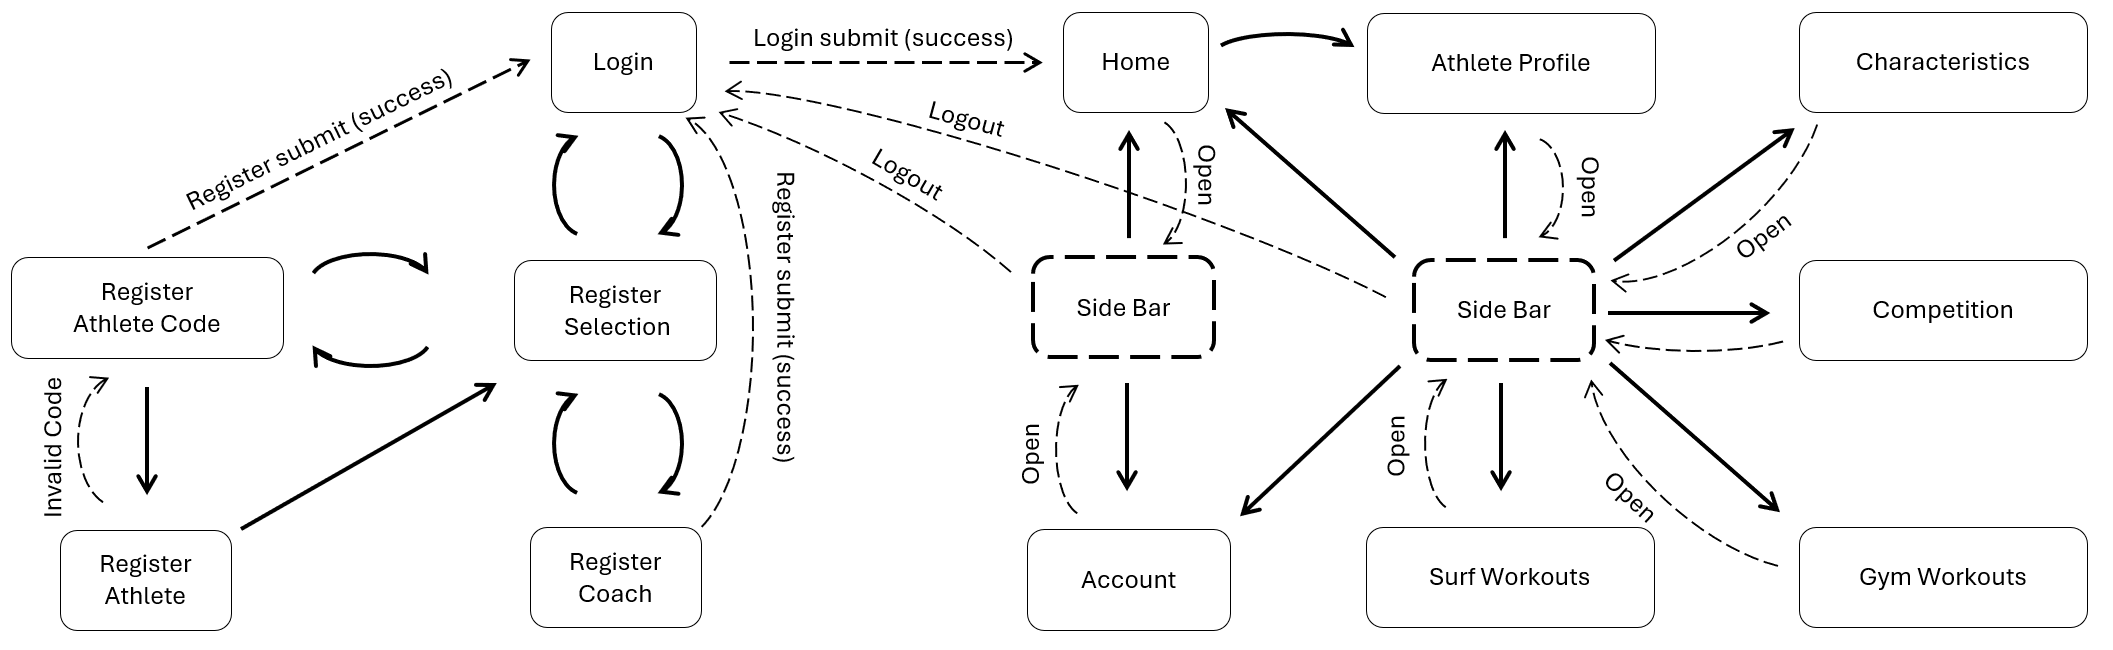
\includegraphics[width=6in]{ViewsDiagram.png}
\caption{Views Diagram}
\end{figure}

The diagram provides an overview of the application's main navigation flow.  
It is divided into two major sections:

\begin{itemize}
\item \textbf{Registration Section}, which includes the Login, Register Selection, Register Coach, Register Athlete Code, and Register Athlete views.
  
\item \textbf{Main Application Section}, which starts with the Home view. From there, the Sidebar component plays a central role in the navigation of the application.  
The Sidebar serves as the main navigation tool, allowing users to easily move between different views.  
Initially, it provides access to the Account view. After an athlete is selected and the user is redirected to the Athlete view, the Sidebar dynamically updates to offer access to views focused on the management of the selected athlete, including Characteristics, Gym Workouts, Surf Workouts, and Competitions.
\end{itemize}


\subsubsection{Functionalities:}
\begin{itemize}
\item User Registration and Login - 
The user registration functionality involves several views: Login, Register Selection, Register Coach, Register Athlete Code, and Register Athlete.
In the Register Selection view, the user chooses between registering as a coach or an athlete.
If the user selects coach, they are redirected directly to the coach registration page.
If the user selects athlete, they are first taken to a page where they must insert their registration code before proceeding to complete their athlete registration.

\item Athlete management - 
The Athlete management functionality is intended for the Home view, meaning the main page. We decided to place athlete management on the main page to provide easier and faster access to athletes, allowing actions such as adding, removing, generating the registration code, and accessing the Athlete view by clicking on their photo, where the athlete’s name and birthdate can then be edited, and also the removing and the generation of the registration code remaining possible. 

\item Athlete Profile - 
This functionality it is related to the Characteristics view. It consists of a chart where it is possible to visualize the athlete’s progress across different aspects, such as height, weight, calories, among others. The chart is clickable, and by clicking on it, users can view the characteristics for the selected date, where they can then edit or delete them. In addition to the chart, the view also displays the most recent characteristics, making it easier for the coach to quickly access the athlete's current condition if they only need a quick overview.

\item Athletes' training records -
In the Athlete view it also provides a quick overview of all workouts, users can browse through all training records and filter them by selecting a specific mesocycle or microcycle, allowing them to view only the workouts within a particular time period.

\end{itemize}

\section{Pending Tasks}
At this stage, among the proposed functional requirements, the remaining tasks are the implementation of athlete training records, that is, water and gym trainings, athlete summaries, and competition records. In addition to these functionalities, an optional feature was also considered: a mobile app that would allow coaches to input athlete records more easily.

\begin{itemize}
\item Athletes' training records - For the implementation of the training records, both gym and water, it is necessary to create backend functionalities to retrieve, create, update, and delete workouts. On the frontend, two views need to be created, one for each type of workout. The Gym Workouts view will include the record of the most recent training session, a table listing all gym workouts — where it will be possible to edit, delete, and navigate to the Gym Workout Details view to access complete workout details — and a button to add a new training session. Similar to the Characteristics view, a quick overview of the latest workout will also be available. In the Surf Workouts view, the structure will be similar to that of the Gym Workouts view, with the addition of the Surf Workout Details view, which will be more detailed, including charts to allow for a more precise analysis of each wave, maneuver, and other surf performance aspects.

\item Athletes' summaries - 

\item Athletes' competition records - Para a implementação dos registos das competições, é tambem necessário 

\item Mobile App (new)
\end{itemize}

% \bibliographystyle{unsrt}
% \bibliography{references}

\end{document}